\section{Specifica Front-End}
	\subsection{SWEDesigner::Client}
		\subsubsection{Informazioni generali}
			\begin{itemize}
          		\item \textbf{Descrizione:}\\
          		Questo package racchiude tutta la componente di Front-end scritta in TypeScript.\\
          		Gli attributi e i metodi di alcune classi saranno definiti a partire dalla prossima versione.
          		\item \textbf{Padre:} SWEDesigner
          		\item \textbf{Package contenuti:}\\
          		\begin{itemize}
          			\item Components\\
          			Questo package contiene tutti i components dell’applicazione
          			\item Services\\
          			Questo package contiene i servizi per le operazioni di iterazione tra i components e
il server
          		\end{itemize}
          	\end{itemize}
	\subsection{SWEDesigner::Client::Components}
		\subsubsection{Informazioni generali}
			\begin{itemize}
          		\item \textbf{Descrizione:}\\
          		Questo package contiene tutti i components dell’applicazione.
          		\item \textbf{Padre:} SWEDesigner::Client
          		\item \textbf{Package contenuti:}\\
          		\begin{itemize}
          			\item Menu\\
          			Il package contiene tutti i components riguardanti la gestione delle funzionalità fornite dal menu.
          			\item Editor\\
          			Il package contiene tutte le components riguardanti l’editor dei diagrammi.
          			\item ActivityFrame\\
          			Il package contiene i components riguardanti la gestione dell’activity frame, per la visione del flusso del programma.
          		\end{itemize}
          	\end{itemize}
		\subsubsection{Classi}
			\paragraph{SWEDesigner::Client::Components::AppComponent}
				\begin{itemize}
          			\item \textbf{Descrizione:}\\
          			Questo component descrive un contenitore per la barra di navigazione e le altre componenti dell’applicazione le quali sono istanziate dinamicamente all’interno del template http.
          			\item \textbf{Utilizzo:}\\
          			AppComponent è il primo component che viene istanziato tramite bootsrap.
          		\end{itemize}
			\paragraph{SWEDesigner::Client::Components::NavbarComponent}
				\begin{itemize}
          			\item \textbf{Descrizione:}\\
          			Questo component permette la navigazione all’interno dell’applicazione tramite links.
          			\item \textbf{Utilizzo:}\\
          			NavbarComponent è istanziato per bootstrap subito dopo dell’AppComponent.
          		\end{itemize}
			\paragraph{SWEDesigner::Client::Components::RegistrationComponent}
				\begin{itemize}
    \item \textbf{Descrizione:}\\
    È il componente che descrive la pagina di registrazione dell’applicazione, mette a disposizione dell’utente un form dove iserire le informazioni necessarie alla creazione di un nuovo account utente. Gestisce le operazioni e la logica applicativa per la registrazione.
    \item \textbf{Utilizzo:}\\
    Questo componente viene istanziato dinamicamente dal servizio Router del framework Angular quando viene richiesta la pagina di registrazione.
	\item \textbf{Metodi:}
    \begin{itemize}
    	\item \emph{-constructor(private router: Router, private accountService: AccountService)}\\
    	Crea un istanziazione di RegistrationComponent
    	\item \textbf{Parametri:}
    		\begin{itemize}
    			\item \emph{-router: Router}
    			Necessario per l'importaziine del Router
    			\item \emph{-accountService: AccountService}
    			Necessario per l'importazione di AccountService
    		\end{itemize}
    	\item \emph{-tryRegistration(e: any)}\\
    	Tenta di registrare un utente
    	\item \textbf{Parametri:}
    		\begin{itemize}
    			\item \emph{+e: any}\\
    			Contiente i dati dell'utente da registrare
    		\end{itemize}
    \end{itemize}
\end{itemize}
			\paragraph{SWEDesigner::Client::Components::LoginComponent}
				\begin{figure}[h!]
	\centering
	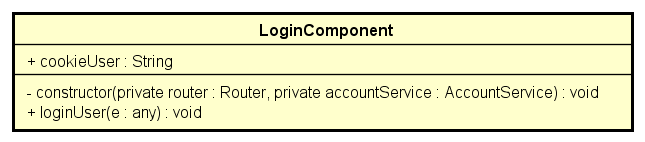
\includegraphics[scale=0.8]{res/sections/SpecificaFrontEnd/Components/Disegnetti/login.png}
	\caption{Diagramma della classe LoginComponent}
\end{figure}

\begin{itemize}
	\item \textbf{Descrizione:}\\
	È il componente che descrive la pagina di login dell’applicazione, mette a disposizione dell’utente un form dove inserire username e password. Gestisce le operazioni e la logica applicativa per il login.
	\item \textbf{Utilizzo:}\\
	Questo componente viene istanziato dinamicamente dal servizio Router del framework Angular quando viene richiesta la pagina di login.
	\item \textbf{Attributi:}
		\begin{itemize}
			\item \emph{+cookieUser: String}\\
			Riceve l'username dai cookie di sessione
		\end{itemize}
	\item \textbf{Metodi:}
		\begin{itemize}
			\item \emph{-constructor(private router: Router, private accountService: AccountService)}\\
    		Crea un istanziazione di RegistrationComponent\\
    		\textbf{Parametri:}
    		\begin{itemize}
    			\item \emph{-router: Router}
    			Necessario per l'importaziine del Router
    			\item \emph{-accountService: AccountService}
    			Necessario per l'importazione di AccountService
    		\end{itemize}
    		\item \emph{+loginUser(e: any)}\\
    		Effettua l'autenticazione dell'utente\\
    		\textbf{Parametri:}
    		\begin{itemize}
    			\item \emph{+e: any}
    			Contiente i dati dell'utente da autenticare
    		\end{itemize}
		\end{itemize}
\end{itemize}
			\paragraph{SWEDesigner::Client::Components::Forgot-pswComponent}
				\begin{itemize}
	\item \textbf{Descrizione:}\\
	È il componente che descrive la pagina per il recupero della password dell'applicazione, mette a disposizione un form in cui inserire l'indirizzo email. Gestisce le operazioni e la logica applicativa relativa al recupero della password.
	\item \textbf{Utilizzo:}\\
	Questo componente viene istanziato dinamicamente dal servizio Router del framework Angular quando viene richiesta la pagina di password dimenticata.
	\item \textbf{Metodi:}
		\begin{itemize}
			\item \emph{-constructor(private accountService: AccountService)}\\
    	Crea un istanziazione di Forgot-pswComponent
    	\item \textbf{Parametri:}
    		\begin{itemize}
    			\item \emph{-accountService: AccountService}
    			Necessario per l'importazione di AccountService
    		\end{itemize}
    		\item \emph{+tryGetNewPassword(e: any)}\\
    		Invia all'utente la password per email
    	\item \textbf{Parametri:}
    		\begin{itemize}
    			\item \emph{+e: any}
    			Contiente i dati dell'utente che ha richiesto il recupero password
    		\end{itemize}
		\end{itemize}
\end{itemize}
	\subsection{SWEDesigner::Client::Components::ActivityFrame}
		\subsubsection{Informazioni generali}
			\begin{itemize}
          		\item \textbf{Descrizione:}\\
          		Questo package contiene i components riguardanti la gestione dell’activity frame, per la visione del flusso del programma.
          		\item \textbf{Padre:} SWEDesigner::Client::Components
          	\end{itemize}
		\subsubsection{Classi}
			\paragraph{SWEDesigner::Client::Components::Editor::ActivityFrame::ActivityFrameComponent}
				\begin{itemize}
          			\item \textbf{Descrizione:}\\
          			Component che descrive la struttura del frame dove l’utente può visualizzare l’activity frame che rappresenta il flusso logico del programma.
          			\item \textbf{Utilizzo:}\\
          			Questo component viene istanziato per bootstrap dopo l’istanziazione del component AppComponent.\
          		\end{itemize}
	\subsection{SWEDesigner::Client::Components::Editor}
		\subsubsection{Informazioni generali}
			\begin{itemize}
          		\item \textbf{Descrizione:}\\
          		Il package contiene tutte le components riguardanti l’editor dei diagrammi.
          		\item \textbf{Padre:} SWEDesigner::Client::Components
          	\end{itemize}
		\subsubsection{Classi}
          	\paragraph{SWEDesigner::Client::Components::Editor::EditorComponent}
          	\begin{figure}[h!]
			\centering
			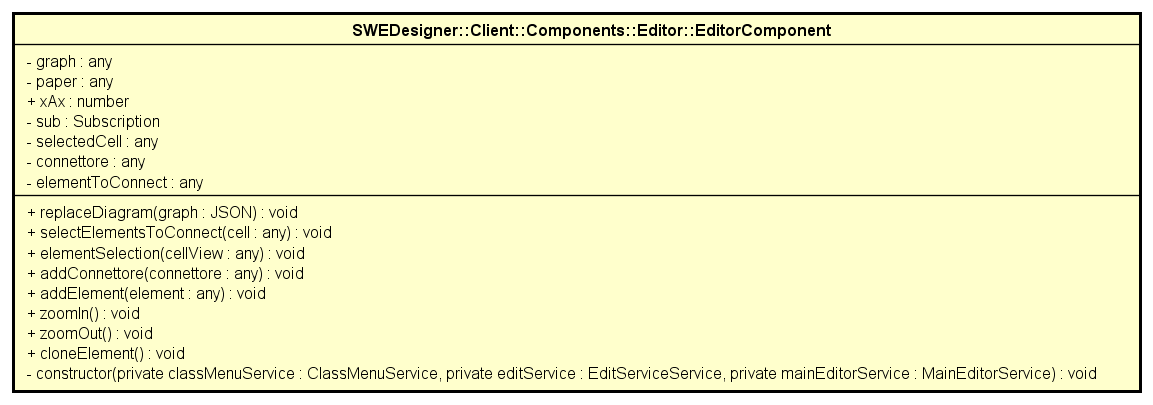
\includegraphics[scale=0.5]{Classi/SWEDesigner__Client__Components__Editor__EditorComponent.png}
			\caption{Diagramma della classe SWEDesigner::Client::Components::Editor::EditorComponent}
 			\end{figure}
				\begin{itemize}
          			\item \textbf{Descrizione:}\\
          			Questo componente contiene la rappresentazione grafica dei diagrammi disegnati dall’utente.
          			\item \textbf{Utilizzo:}\\
          			Questo componente viene instanziato dinamicamente dal servizio Router del framework Angular quando viene richiesta la pagina dell’editor diagrammi.
          			\item \textbf{Attributi:}\\
          			\begin{itemize}
          				\item \emph{-graph: any}\\
            			Contiene tutti gli elementi del grafico
            			\item \emph{-paper: any}\\
            			Assicura che vengano renderizzati gli elementi del grafico
            			\item \emph{+xAx: number}\\
            			Serve per scalare il grafico
            			\item \emph{-sub: Subscription}\\
            			Permette la funzione di zoom
            			\item \emph{-selectedCell: any}\\
            			Punta all'elemento selezionato con il click
            			\item \emph{-connettore: any}\\
            			Il tipo del connettore selezionato
            			\item \emph{-elementToConnect: any}\\
            			Punta all'elemento selezionato con il click, che sarà collegato con il connettore
          			\end{itemize}
          			\item \textbf{Metodi:}\\
          			\begin{itemize}
          				\item \emph{-constructor(private classMenuService: ClassMenuService, private editService: EditServiceService, private mainEditorService: MainEditorService): void}\\
          				Questo metodo è il costruttore della classe
          				\item \textbf{Parametri:}\\
            				\begin{itemize}
            					\item \emph{private classMenuService: ClassMenuService}\\
            					Service ClassMenuService
            					\item \emph{private editService: EditServiceService}\\
            					Service EditServiceService
            					\item \emph{private mainEditorService: MainEditorService}\\
            					Service MainEditorService
            				\end{itemize}
          				\item \emph{+replaceDiagram(graph: JSON): void}\\
          				Questo metodo viene utilizzato per rimpiazzare l'editor con una nuova finestra contenuta nel file JSON
          				\item \textbf{Parametri:}\\
            				\begin{itemize}
            					\item \emph{graph: JSON}\\
            					Grafico da aprire in formato JSON
            				\end{itemize}
          				\item \emph{+selectElementsToConnect(cell: any): void}\\
          				Questo metodo viene utilizzato per selezionare gli elementi da collegare con il connettore selezionato
          				\item \textbf{Parametri:}\\
            				\begin{itemize}
            					\item \emph{cell: any}\\
            					Elemento selezionato
            				\end{itemize}
            			\item \emph{+elementSelection(cellView: any): void}\\
            			Questo metodo seleziona un elemento nell'editor
            			\item \textbf{Parametri:}\\
            				\begin{itemize}
            					\item \emph{cellView: any}\\
            					Elemento selezionato
            				\end{itemize}
            			\item \emph{+addConnettore(connettore: any): void}\\
            			Aggiunge il connettore alla classe
            			\item \textbf{Parametri:}\\
            				\begin{itemize}
            					\item \emph{connettore: any}\\
            					Connettore da aggiungere
            				\end{itemize}
            			\item \emph{+addElement(element: any): void}\\
            			Questo metodo aggiunge un elemento all'editor
            			\item \textbf{Parametri:}\\
            				\begin{itemize}
            					\item \emph{element: any}\\
            					Elemento da aggiungere all'editor
            				\end{itemize}
            			\item \emph{+zoomIn(): void}\\
            			Questo metodo incrementa la scala dell'editor
            			\item \emph{+zoomOut(): void}\\
            			Questo metodo decrementa la scala dell'editor
            			\item \emph{+cloneElement(): void}\\
            			Questo metodo clona l'elemento selezionato
          			\end{itemize}
          		\end{itemize}
          	\paragraph{SWEDesigner::Client::Components::Editor::ClassMenuComponent}
          	\begin{figure}[h!]
			\centering
			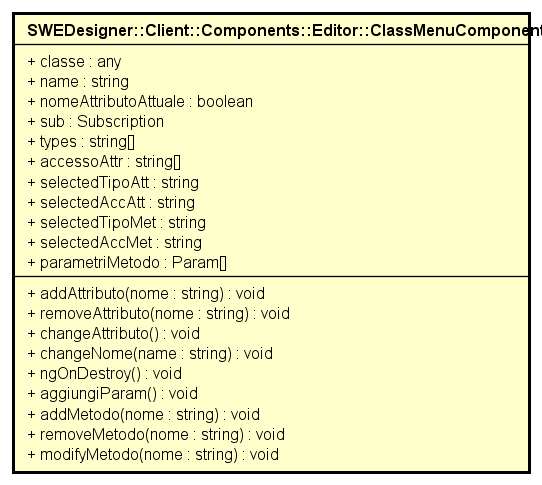
\includegraphics[scale=0.8]{Classi/SWEDesigner__Client__Components__Editor__ClassMenuComponent.png}
			\caption{Diagramma della classe SWEDesigner::Client::Components::Editor::ClassMenuComponent}
 			\end{figure}
				\begin{itemize}
          			\item \textbf{Descrizione:}\\
          			Questo component permette la modifica dei campi dati di un oggetto selezionato nell’editorComponent.
          			\item \textbf{Utilizzo:}\\
          			Questo component è figlio di editorComponent viene visualizzato quando viene selezionato un elemento editabile nell’editorComponent.
          			\item \textbf{Attributi:}\\
          			\begin{itemize}
          				\item \emph{+classe: any}\\
            			La classe correntemente selezionata dell'EditorComponent
            			\item \emph{+name: string}\\
            			Il nome della classe correntemente selezionata
            			\item \emph{+nomeAttributoAttuale: boolean}\\
            			True se il nome del nuovo attributo è uguale all'attributo attuale
            			\item \emph{+sub: Subscription}\\
            			Subscription dell'oggetto observable
            			\item \emph{+types: string[]}\\
            			Array contenente i tipi di dato primitivi
            			\item \emph{+accessoAttr: string[]}\\
            			Array contenente i tipi di accesso
            			\item \emph{+selectedTipoAtt: string}\\
            			Memorizza il tipo selezionato per il costruttore del nuovo attributo
            			\item \emph{+selectedAccAtt: string}\\
            			Memorizza la visibilità selezionata per creare un nuovo attributo
            			\item \emph{+selectedTipoMet: string}\\
            			Memorizza il tipo di ritorno per costruire un nuovo metodo
            			\item \emph{+selectedAccMet: string}\\
            			Memorizza il tipo di visibilità per costruire un nuovo metodo
            			\item \emph{+parametriMetodo: Param[]}\\
            			Memorizza un array di parametri per costruire un nuovo metodo
          			\end{itemize}
          			\item \textbf{Metodi:}\\
          			\begin{itemize}
          				\item \emph{+addAttributo(nome: string): void}\\
            			Aggiunge un attributo alla classe
            			\item \textbf{Parametri:}\\
            				\begin{itemize}
            					\item \emph{nome: string}\\
            					Nome del nuovo attributo
            				\end{itemize}
            			\item \emph{+removeAttributo(nome: string): void}\\
            			Rimuove un attributo dalla classe
            			\item \textbf{Parametri:}\\
            				\begin{itemize}
            					\item \emph{nome: string}\\
            					Nome dell'attributo da eliminare
            				\end{itemize}
            			\item \emph{+changeAttributo(): void}\\
            			Modifica le proprietà di un attributo
            			\item \emph{+changeNome(name: string): void}\\
            			Modifica il nome della classe
            			\item \textbf{Parametri:}\\
            				\begin{itemize}
            					\item \emph{name: string}\\
            					Nuovo nome della classe
            				\end{itemize}
            			\item \emph{+ngOnDestroy(): void}\\
            			Previene memory leak quando il componente è distrutto
            			\item \emph{+aggiungiParam(): void}\\
            			Aggiunge un nuovo parametri nell'array dei parametri
            			\item \emph{+addMetodo(nome: string): void}\\
            			Aggiunge un nuovo metodo alla classe
            			\item \textbf{Parametri:}\\
            				\begin{itemize}
            					\item \emph{nome: string}\\
            					Nome del metodo
            				\end{itemize}
            			\item \emph{+removeMetodo(nome: string): void}\\
            			Rimuove un metodo dalla classe
            			\item \textbf{Parametri:}\\
            				\begin{itemize}
            					\item \emph{nome: string}\\
            					Nome del metodo da rimuovere
            				\end{itemize}
            			\item \emph{+modifyMetodo(nome: string): void}\\
            			Fa entrare l'editor in modalità Activity per modificare il corpo del metodo
            			\item \textbf{Parametri:}\\
            				\begin{itemize}
            					\item \emph{nome: string}\\
            					Nome del metodo da modificare
            				\end{itemize}
          			\end{itemize}
          		\end{itemize}
			\paragraph{SWEDesigner::Client::Components::Editor::ToolbarComponent}
			\begin{figure}[h!]
			\centering
			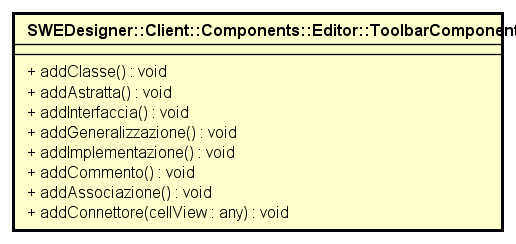
\includegraphics[scale=0.8]{Classi/SWEDesigner__Client__Components__Editor__ToolbarComponent.png}
			\caption{Diagramma della classe SWEDesigner::Client::Components::Editor::ToolbarComponent}
 			\end{figure}
				\begin{itemize}
          			\item \textbf{Descrizione:}\\
          			La classe si occupa di fornire una toolbar per l'inserimento degli elementi del diagramma delle attività o del diagramma delle classi.
          			\item \textbf{Utilizzo:}\\
          			Ogni volta che viene selezionato un elemento esso viene inserito sul grafico. Nel caso dei connettori occorre selezionare, successivamente al connettore, i due elementi da collegare.
          			\item \textbf{Metodi:}\\
          			\begin{itemize}
          				\item \emph{+addClasse(): void}\\
          				Il metodo aggiunge una classe di nome "Classe" nell'area di disegno;
          				\item \emph{+addAstratta(): void}\\
          				Il metodo aggiunge una classe astratta di nome "ClasseAstratta" nell'area di disegno;
          				\item \emph{+addInterfaccia(): void}\\
          				Il metodo aggiunge un interfaccia di nome "Interfaccia" nell'area di disegno;
          				\item \emph{+addGeneralizzazione(): void}\\
          				Il metodo seleziona il tipo di connettore "Generalizzazione";
          				\item \emph{+addImplementazione(): void}\\
          				Il metodo seleziona il tipo di connettore "Implementazione";
          				\item \emph{+addCommento(): void}\\
          				Il metodo aggiunge un elemento di tipo "Commento" nell'area di disegno;
          				\item \emph{+addAssociazione(): void}\\
          				Il metodo seleziona il tipo di connettore "Associazione";
          				\item \emph{+addConnettore(cellView: any): void}\\
          				Il metodo serve, in caso venga selezionato un connettore, a selezionare i due elementi da collegare con il connettore selezionato con uno dei metodi precedenti.
          				\item \textbf{Parametri:}\\
            				\begin{itemize}
            					\item \emph{cellView: any}\\
            					Elemento da selezionare per essere collegato con il connettore selezionato
            				\end{itemize}
          			\end{itemize}
          		\end{itemize}
	\subsection{SWEDesigner::Client::Components::Menu}
		\subsubsection{Informazioni generali}
			\begin{itemize}
          		\item \textbf{Descrizione:}\\
          		Il package contiene tutti i components riguardanti la gestione delle funzionalità fornite dal menu.
          		\item \textbf{Padre:} SWEDesigner::Client::Components
          	\end{itemize}
		\subsubsection{Classi}
			\paragraph{SWEDesigner::Client::Components::Menu::MenuComponent}
				\begin{itemize}
          			\item \textbf{Descrizione:}\\
          			Component che contiene l’insieme di funzionalità fornite all’utente per la gestione dei progetti, dei propri dati personali, e della rappresentazione dei grafici su cui sta lavorando.
          			\item \textbf{Utilizzo:}\\
          			Component che viene istanziato per bootstrap dopo che è stato istanziato il component appComponent.
          		\end{itemize}
			\paragraph{SWEDesigner::Client::Components::Menu::FileComponent}
				\begin{itemize}
          			\item \textbf{Descrizione:}\\
          			Component che contiene l’insieme di funzionalità fornite all’utente per la gestione del progetto attualmente in uso.
          			\item \textbf{Utilizzo:}\\
          			Component che viene istanziato per bootstrap dopo che è stato istanziato il component menuComponent.
          		\end{itemize}
			\paragraph{SWEDesigner::Client::Components::Menu::LayerComponent}
				\begin{itemize}
          			\item \textbf{Descrizione:}\\
          			Component che contiene l’insieme di funzionalità fornite all’utente per la gestione dei layer del progetto in uso.
          			\item \textbf{Utilizzo:}\\
          			Component che viene istanziato per bootstrap dopo che è stato istanziato il component menuComponent.
          		\end{itemize}
			\paragraph{SWEDesigner::Client::Components::Menu::ProgettoComponent}
				\begin{itemize}
          			\item \textbf{Descrizione:}\\
          			Component che contiene l’insieme di funzionalità fornite all’utente per la gestione dei propri progetti salvati.
          			\item \textbf{Utilizzo:}\\
          			progettoComponent viene istanziato per bootstrap dopo che è stato istanziato il component menuComponent.
          		\end{itemize}
			\paragraph{SWEDesigner::Client::Components::Menu::ProfiloComponent}
				\begin{itemize}
          			\item \textbf{Descrizione:}\\
          			Component che contiene l’insieme di funzionalità fornite all’utente per la gestione dei propri dati personali.
          			\item \textbf{Utilizzo:}\\
          			Component che viene istanziato per bootstrap dopo che è stato istanziato il component menuComponent.
          		\end{itemize}
			\paragraph{SWEDesigner::Client::Components::Menu::ModificaComponent}
			\begin{figure}[h!]
			\centering
			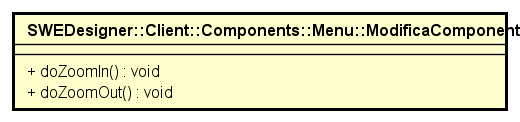
\includegraphics[scale=0.8]{Classi/SWEDesigner__Client__Components__Menu__ModificaComponent.png}
			\caption{Diagramma della classe SWEDesigner::Client::Components::Menu::ModificaComponent}
 			\end{figure}
				\begin{itemize}
          			\item \textbf{Descrizione:}\\
          			Component che contiene l’insieme di funzionalità fornite all’utente per la modifica del progetto in uso, come ad esempio effettuare lo zoom, oppure eliminare o copiare un elemento selezionato.
          			\item \textbf{Utilizzo:}\\
          			Component che viene istanziato per bootstrap dopo che è stato istanziato il component menuComponent.
          			\item \textbf{Metodi:}\\
          			\begin{itemize}
          				\item \emph{+doZoomIn(): void}
          				Esegue lo zoomIn
          				\item \emph{+doZoomOut(): void}
          				Esegue lo zoomOut
          			\end{itemize}
          		\end{itemize}
          	\paragraph{SWEDesigner::Client::Components::Menu::TemplateComponent}
				\begin{itemize}
          			\item \textbf{Descrizione:}\\
          			Component che contiene l’insieme di funzionalità fornite all’utente per l’importazione e gestione dei template.
          			\item \textbf{Utilizzo:}\\
          			Component che viene istanziato per bootstrap dopo che è stato istanziato il component menuComponent.
          		\end{itemize}
    \subsection{SWEDesigner::Client::Services}
		\subsubsection{Informazioni generali}
			\begin{itemize}
          		\item \textbf{Descrizione:}\\
          		Il package contiene i servizi per le operazioni di iterazione tra i component e il server.
          		\item \textbf{Padre:} SWEDesigner::Client
          		\item \textbf{Package contenuti:}\\
          		\begin{itemize}
          			\item Models\\
          			Il package contiene moduli necessari a storicizzare i dati inseriti all’interno dei diagrammi.
          		\end{itemize}
          	\end{itemize}
		\subsubsection{Classi}
			\paragraph{SWEDesigner::Client::Services::MenuService}
			\begin{figure}[h!]
			\centering
			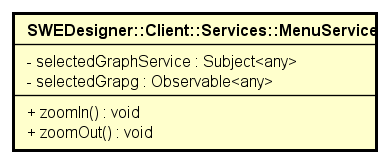
\includegraphics[scale=0.8]{Classi/SWEDesigner__Client__Services__MenuService.png}
			\caption{Diagramma della classe SWEDesigner::Client::Services::MenuService}
 			\end{figure}
				\begin{itemize}
          			\item \textbf{Descrizione:}\\
          			Classe che definisce i metodi per le operazioni fornite all’utente dal menu.
          			\item \textbf{Utilizzo:}\\
          			É istaziata dal framework Angular e i suoi metodi sono utilizzati dal component menuComponent.
          			\item \textbf{Attributi:}\\
          			\begin{itemize}
          				\item \emph{-selectedGraphService: Subject<any>}\\
          				\item \emph{-selectedGrapg: Observable<any>}\\
          			\end{itemize}
          			\item \textbf{Metodi:}\\
          			\begin{itemize}
          				\item \emph{+zoomIn(): void}\\
          				Aumenta la dimensione degli oggetti nell'editor
          				\item \emph{+zoomOut(): void}\\
          				Diminuisce la dimensione degli oggetti nell'editor
          			\end{itemize}
          		\end{itemize}
          	\paragraph{SWEDesigner::Client::Services::MainEditorService}
          	\begin{figure}[h!]
			\centering
			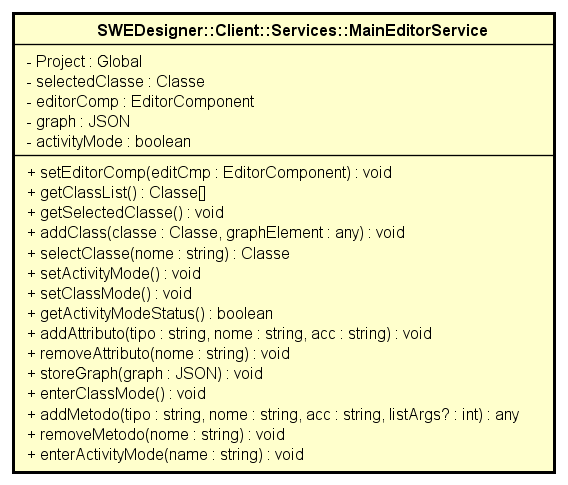
\includegraphics[scale=0.8]{Classi/SWEDesigner__Client__Services__MainEditorService.png}
			\caption{Diagramma della classe SWEDesigner::Client::Services::MainEditorService}
 			\end{figure}
				\begin{itemize}
          			\item \textbf{Descrizione:}\\
          			Classe che definisce i metodi per le operazioni all’interno dei diagrammi e la comunicazione tra componenti e server.
          			\item \textbf{Utilizzo:}\\
          			É istaziata dal framework Angular e i suoi metodi sono utilizzati dai component editorComponent e classMenuComponent.
          			\item \textbf{Attributi:}\\
          			\begin{itemize}
          				\item \emph{-Project: Global}\\
          				Si utilizza per memorizzare e recuperare informazione riguardo il progetto corrente
          				\item \emph{-selectedClasse: Classe}\\
          				Memorizza la classe corrispondente di tipo "Classe" della classe selezionata nel canvas dell'editor
          				\item \emph{-editorComp: EditorComponent}\\
          				Si utilizza per accedere direttamente all'EditorComponent
          				\item \emph{-graph: JSON}\\
          				Si utilizza per per salvare il grafico dell'editor
          				\item \emph{-activityMode: boolean}\\
          				Indica se il diagramma delle attività è in uso
          			\end{itemize}
          			\item \textbf{Metodi:}\\
          			\begin{itemize}
          				\item \emph{+setEditorComp(editCmp: EditorComponent): void}\\
          				Questo metodo viene usato per l'istanziazione dell'EditorComponent come proprietà interna di questa classe
          				\item \textbf{Parametri:}\\
            				\begin{itemize}
            					\item \emph{editCmp: EditorComponent}\\
            					L'istanza dell'EditorComponent
            				\end{itemize}
          				\item \emph{+getClassList(): Classe[]}\\
          				Questo metodo viene usato per richiamare l'array di classi presente nel progetto
          				\item \emph{+getSelectedClasse(): void}\\
          				Questo metodo ritorna la classe selezionata di tipo "Classe"
          				\item \emph{+addClass(classe: Classe, graphElement: any): void}\\
          				Questo metodo aggiunge un oggetto di tipo classe nell'array di classi del progetto
          				\item \textbf{Parametri:}\\
            				\begin{itemize}
            					\item \emph{classe: Classe}\\
            					Questo oggetto è una rappresentazione, di tipo "Classe" o "ClasseAstratta", del parametro graphelement
            					\item \emph{graphElement: any}\\
            					Questo è un elemento della libreria grafica JointJs
            				\end{itemize}
          				\item \emph{+selectClasse(nome: string): Classe}\\
          				Questo metodo cerca, all'interno della collezione di classi del progetto, una classe con lo stesso nome di quello fornito come parametro
          				\item \textbf{Parametri:}\\
            				\begin{itemize}
            					\item \emph{nome: string}\\
            					Nome della classe da cercare
            				\end{itemize}
          				\item \emph{+setActivityMode(): void}\\
          				Questo metodo setta a True il valore di activityMode
          				\item \emph{+setClassMode(): void}\\
          				Questo metodo setta a False il valore di activityMode
          				\item \emph{+getActivityModeStatus(): boolean}\\
          				Questo metodo ritorna il valore di activityMode
          				\item \emph{+addAttributo(tipo: string, nome: string, acc: string): void}\\
          				Questo metodo richiama il metodo addAttributo della "selectedClasse"
          				\item \textbf{Parametri:}\\
            				\begin{itemize}
            					\item \emph{tipo: string}\\
            					Il tipo dell'attributo da aggiungere con addAttributo
            					\item \emph{nome: string}\\
            					Il nome dell'attributo da aggiungere con addAttributo
            					\item \emph{acc: string}\\
            					La visibilità dell'attributo da aggiungere con addAttributo
            				\end{itemize}
            			\item \emph{+removeAttributo(nome: string): void}\\
          				Questo metodo richiama il metodo removeAttr della "selectedClasse"
          				\item \textbf{Parametri:}\\
            				\begin{itemize}
            					\item \emph{nome: string}\\
            					Il nome dell'attributo da rimuovere
            				\end{itemize}
            			\item \emph{+storeGraph(graph: JSON): void}\\
          				Questo metodo salva in "this.graph" il grafico passato come parametro
          				\item \textbf{Parametri:}\\
            				\begin{itemize}
            					\item \emph{graph: JSON}\\
            					Un grafico in formato JSON
            				\end{itemize}
            			\item \emph{+enterClassMode(): void}\\
          				Questo metodo viene utilizzato per ripristinare il diagramma delle classi memorizzato in "this.graph"
          				\item \emph{+addMetodo(tipo: string, nome: string, acc: string, listArgs?: any): void}\\
          				Questo metodo aggiunge un nuovo metodo alla "selectedClasse"
          				\item \textbf{Parametri:}\\
            				\begin{itemize}
            					\item \emph{tipo: string}\\
            					Tipo di ritorno del metodo
            					\item \emph{nome: string}\\
            					Nome del metodo
            					\item \emph{acc: string}\\
            					La visibilità del metodo
            					\item \emph{listArgs?: any}\\
            					Lista dei parametri del metodo, se ce ne sono
            				\end{itemize}
            			\item \emph{+removeMetodo(nome: string): void}\\
          				Questo metodo richiama il metodo removeMetodo della "selectedClasse"
          				\item \textbf{Parametri:}\\
            				\begin{itemize}
            					\item \emph{nome: string}\\
            					Nome del metodo da eliminare
            				\end{itemize}
            			\item \emph{+enterActivityMode(name: string): void}\\
          				Questo metodo cerca un metodo nella "selectedClasse" e recupera il suo diagramma per chiamare il metodo replaceDiagram dell'editorComp, il quale carica i metodi del diagramma in Canvas
          				\item \textbf{Parametri:}\\
            				\begin{itemize}
            					\item \emph{name: string}\\
            					Nome del metodo da trovare
            				\end{itemize}
          			\end{itemize}
          		\end{itemize}
          	\paragraph{SWEDesigner::Client::Services::ToolbarService}
				\begin{itemize}
          			\item \textbf{Descrizione:}\\
          			Classe che definisce i metodi per le operazioni di inserimento di nuovi elementi all’interno dell’editor di diagrammi.
          			\item \textbf{Utilizzo:}\\
          			É istaziata dal framework Angular e i suoi metodi sono utilizzati dal component editorComponent.
          		\end{itemize}
          	\paragraph{SWEDesigner::Client::Services::ActivityFrameService}
				\begin{itemize}
          			\item \textbf{Descrizione:}\\
          			Classe che definisce i metodi per le operazioni di navigazione tra i metodi all’interno dell’activity frame.
          			\item \textbf{Utilizzo:}\\
          			É istaziata dal framework Angular e i suoi metodi sono utilizzati dal component activityFrameComponent.
          		\end{itemize}
          	\paragraph{SWEDesigner::Client::Services::ClassMenuService}
          	\begin{figure}[h!]
			\centering
			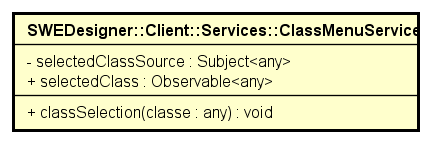
\includegraphics[scale=0.8]{Classi/SWEDesigner__Client__Services__ClassMenuService.png}
			\caption{Diagramma della classe SWEDesigner::Client::Services::ClassMenuService}
 			\end{figure}
				\begin{itemize}
          			\item \textbf{Descrizione:}\\
          			Classe che definisce i metodi per le operazioni di modifica di un elemento selezionato all’interno del diagramma rappresentato.
          			\item \textbf{Utilizzo:}\\
          			É istaziata dal framework Angular e i suoi metodi sono utilizzati dal component classMenuService.
          			\item \textbf{Attributi:}\\
          			\begin{itemize}
          				\item \emph{-selectedClassSource: Subject<any>}\\
            			Subject della classe selezionata
            			\item \emph{+selectedClass: Observable<any>}\\
            			Observable della classe selezionata
          			\end{itemize}
          			\item \textbf{Metodi:}\\
          			\begin{itemize}
          				\item \emph{+classSelection(classe: any): void}\\
            			Aggiorna il subject della classe
          			\end{itemize}
          		\end{itemize}
          	\paragraph{SWEDesigner::Client::Services::AccountService}
				\begin{itemize}
          			\item \textbf{Descrizione:}\\
          			Classe che definisce i metodi di registrazione, login e recupero dati utente dal server.
          			\item \textbf{Utilizzo:}\\
          			É istaziata dal framework Angular e i suoi metodi sono utilizzati dai component registrationComponent e loginComponent.
          		\end{itemize}
	\subsection{SWEDesigner::Client::Services::Models}
		\subsubsection{Informazioni generali}
			\begin{itemize}
          		\item \textbf{Descrizione:}\\
          		Il package contiene moduli necessari a storicizzare i dati inseriti all’interno
dei diagrammi.
          		\item \textbf{Padre:} SWEDesigner::Client::Services
          	\end{itemize}
		\subsubsection{Classi}
			\paragraph{SWEDesigner::Client::Services::Param}
			\begin{figure}[h!]
			\centering
			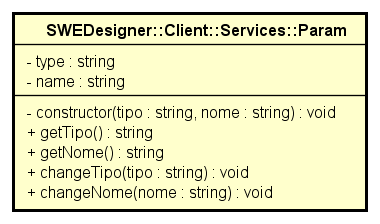
\includegraphics[scale=0.8]{Classi/SWEDesigner__Client__Services__Param.png}
			\caption{Diagramma della classe SWEDesigner::Client::Services::Param}
 			\end{figure}
				\begin{itemize}
          			\item \textbf{Descrizione:}\\
          			Classe che definisce i metodi di settaggio e richiesta dei parametri nome e tipo.
          			\item \textbf{Utilizzo:}\\
          			É istaziata dal framework Angular e i suoi metodi sono utilizzati dal model attributo.
          			\item \textbf{Attributi:}\\
          			\begin{itemize}
          				\item \emph{-type: string}\\
            			Tipo del parametro
            			\item \emph{-name: string}\\
            			Nome del parametro
          			\end{itemize}
          			\item \textbf{Metodi:}\\
          			\begin{itemize}
          				\item \emph{-constructor(tipo: string, nome: string): void}\\
            			Costruttore
            			\item \textbf{Parametri:}\\
            				\begin{itemize}
            					\item \emph{tipo: string}\\
            					Tipo del parametro
            					\item \emph{nome: string}\\
            					Nome del parametro
            				\end{itemize}
            			\item \emph{+getTipo(): string}\\
            			Ritorna il tipo del parametro
            			\item \emph{+getNome(): string}\\
            			Ritorna il nome del parametro
            			\item \emph{+changeTipo(tipo: string): void}\\
            			Modifica il tipo del parametro
            			\item \textbf{Parametri:}\\
            				\begin{itemize}
            					\item \emph{tipo: string}\\
            					Nuovo tipo
            				\end{itemize}
            			\item \emph{+changeNome(nome: string): void}\\
            			Modifica il nome del parametro
            			\item \textbf{Parametri:}\\
            				\begin{itemize}
            					\item \emph{nome: string}\\
            					Nuovo nome
            				\end{itemize}
          			\end{itemize}
          		\end{itemize}
          	\paragraph{SWEDesigner::Client::Services::Attributo}
          	\begin{figure}[h!]
			\centering
			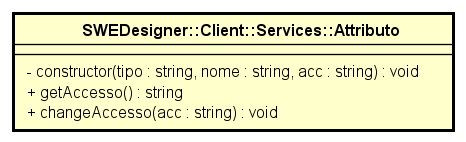
\includegraphics[scale=0.8]{Classi/SWEDesigner__Client__Services__Attributo.png}
			\caption{Diagramma della classe SWEDesigner::Client::Services::Attributo}
 			\end{figure}
				\begin{itemize}
          			\item \textbf{Descrizione:}\\
          			Classe derivata da Param che definisce i metodi di settaggio e richiesta dei parametri di visibilità.
          			\item \textbf{Utilizzo:}\\
          			É istaziata dal framework Angular e i suoi metodi sono utilizzati dal model classe.
          			\item \textbf{Metodi:}\\
          				\item \emph{-constructor (tipo: string, nome: string, acc: string): void}\\
          				Costruttore
          				\item \textbf{Parametri:}\\
            				\begin{itemize}
            					\item \emph{tipo: string}\\
            					Tipo dell'attributo
            					\item \emph{nome: string}\\
            					Nome dell'attributo
            					\item \emph{acc: string}\\
            					Accessibilità dell'attributo
            				\end{itemize}
            			\item \emph{+getAccesso(): string}\\
          				Rstituisce l'accessibilità dell'attributo
          				\item \emph{+changeAccesso(acc: string): void}\\
          				Modifica l'accessibilità dell'attributo
          				\item \textbf{Parametri:}\\
            				\begin{itemize}
            					\item \emph{acc: string}\\
            					Nuova accessibilità
            				\end{itemize}
          		\end{itemize}
          	\paragraph{SWEDesigner::Client::Services::Metodo}
          	\begin{figure}[h!]
			\centering
			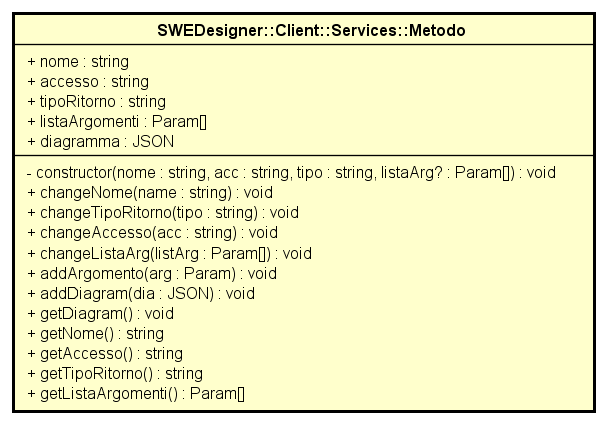
\includegraphics[scale=0.8]{Classi/SWEDesigner__Client__Services__Metodo.png}
			\caption{Diagramma della classe SWEDesigner::Client::Services::Metodo}
 			\end{figure}
				\begin{itemize}
          			\item \textbf{Descrizione:}\\
          			Classe che definisce i metodi di settaggio e richiesta dei metodi definiti all’interno dei diagrammi.
          			\item \textbf{Utilizzo:}\\
          			É istaziata dal framework Angular e i suoi metodi sono utilizzati dal model classe.
          			\item \textbf{Attributi:}\\
          			\begin{itemize}
          				\item \emph{+nome: string}\\
            			Nome del metodo
            			\item \emph{+accesso: string}\\
            			Visibilità del metodo
            			\item \emph{+tipoRitorno: string}\\
            			Tipo di ritorno del metodo
            			\item \emph{+listaArgomenti: Param[]}\\
            			Lista argomenti del metodo
            			\item \emph{+diagramma: JSON}\\
            			Definisce il metodo corrente in JSON
          			\end{itemize}
          			\item \textbf{Metodi:}\\
          			\begin{itemize}
          				\item \emph{-constructor(nome: string, acc: string, tipo: string, listaArg?: Param[]): void}\\
          				Costruttore
          				\item \textbf{Parametri:}\\
            				\begin{itemize}
            					\item \emph{nome: string}\\
            					Nome del metodo
            					\item \emph{acc: string}\\
            					Visibilità del metodo
            					\item \emph{tipo: string}\\
            					Tipo di ritorno del metodo
            					\item \emph{listaArg?: Param[]}\\
            					Lista argomenti del metodo
            				\end{itemize}
          				\item \emph{+changeNome(name: string): void}\\
          				Modifica il nome del metodo
          				\item \textbf{Parametri:}\\
            				\begin{itemize}
            					\item \emph{name: string}\\
            					Nuovo nome del metodo
            				\end{itemize}
          				\item \emph{+changeTipoRitorno(tipo: string): void}\\
          				Modifica il tipo di ritorno del metodo
          				\item \textbf{Parametri:}\\
            				\begin{itemize}
            					\item \emph{tipo: string}\\
            					Nuovo tipo di ritorno del metodo
            				\end{itemize}
          				\item \emph{+changeAccesso(acc: string): void}\\
          				Modifica la visibilità del metodo
          				\item \textbf{Parametri:}\\
            				\begin{itemize}
            					\item \emph{acc: string}\\
            					Nuova visibilità del metodo
            				\end{itemize}
          				\item \emph{+changeListaArg(listArg: Param[]): void}\\
          				 Cambia il riferimento all'array dei parametri formali
          				 \item \textbf{Parametri:}\\
            				\begin{itemize}
            					\item \emph{listArg: Param[]}\\
            					Array dei parametri
            				\end{itemize}
          				\item \emph{+addArgomento(arg: Param) : void}\\
          				Aggiunge un nuovo parametro al metodo
          				\item \textbf{Parametri:}\\
            				\begin{itemize}
            					\item \emph{arg: Param}\\
            					Parametro
            				\end{itemize}
          				\item \emph{+addDiagram(dia: JSON): void}\\
          				Assegna il file JSON al diagramma degli attributi
          				\item \textbf{Parametri:}\\
            				\begin{itemize}
            					\item \emph{dia: JSON}\\
            					File JSON
            				\end{itemize}
          				\item \emph{+getDiagram(): void}\\
          				Ritorna il diagramma del metodo
          				\item \emph{+getNome(): string}\\
          				Ritorna il nome del metodo
          				\item \emph{+getAccesso(): string}\\
          				Ritorna il tipo di visibilità del metodo
          				\item \emph{+getTipoRitorno(): string}\\
          				Ritorna il tipo di ritorno del metodo
          				\item \emph{+getListaArgomenti(): Param[]}\\
          				Ritorna l'array degli argomenti
            		\end{itemize}
          		\end{itemize}
          	\paragraph{SWEDesigner::Client::Services::Classe}
          	\begin{figure}[h!]
			\centering
			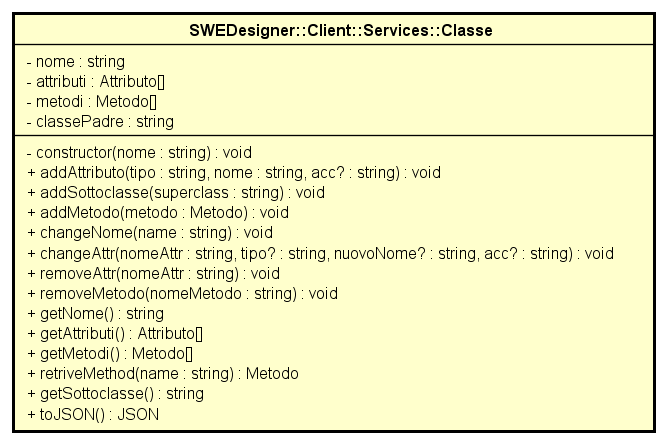
\includegraphics[scale=0.8]{Classi/SWEDesigner__Client__Services__Classe.png}
			\caption{Diagramma della classe SWEDesigner::Client::Services::Classe}
 			\end{figure}
				\begin{itemize}
          			\item \textbf{Descrizione:}\\
          			Classe che definisce i metodi di settaggio e richiesta di tutti gli elementi che sono contenuti in una classe. Contiene un array di metodi, con le relative rappresentazioni grafiche dei metodi implementati, e un array di attributi, oltre ai campi utili all’identificazione della classe.
          			\item \textbf{Utilizzo:}\\
          			É istaziata dal framework Angular e i suoi metodi sono utilizzati dal model global.
          			\item \textbf{Attributi:}\\
          			\begin{itemize}
          				\item \emph{-nome: string}\\
            			Il nome della classe
            			\item \emph{-attributi: Attributo[]}\\
            			Array di attributi della classe
            			\item \emph{-metodi: Metodo[]}\\
            			Array di metodi della classe
            			\item \emph{-classePadre: string}\\
            			La classe estesa da questa classe
          			\end{itemize}
          			\item \textbf{Metodi:}\\
          			\begin{itemize}
          				\item \emph{-constructor(nome: string): void}\\
            			Costruisce un nuovo oggetto di tipo classe e gli assegna un nome
            			\item \textbf{Parametri:}\\
            				\begin{itemize}
            					\item \emph{nome: string}\\
            					Nome della classe
            				\end{itemize}
            			\item \emph{+addAttributo(tipo: string, nome: string, acc?: string): void}\\
            			Aggiunge un nuovo attribuo alla lista degli attributi dopo aver controllato che non ne esista già uno con lo stesso nome
            			\item \textbf{Parametri:}\\
            				\begin{itemize}
            					\item \emph{tipo: string}\\
            					Tipo del nuovo attributo
            					\item \emph{nome: string}\\
            					Nome del nuovo attributo
            					\item \emph{acc?: string}\\
            					Visibilità dell'attributo
            				\end{itemize}
            			\item \emph{+addSottoclasse(superclass: string): void}\\
            			Inserisce il nome della classe che questa classe estende
            			\item \textbf{Parametri:}\\
            				\begin{itemize}
            					\item \emph{superclass: string}\\
            					Nome della classe padre
            				\end{itemize}
            			\item \emph{+addMetodo(metodo: Metodo): void}\\
            			Aggiunge un nuovo metodo
            			\item \textbf{Parametri:}\\
            				\begin{itemize}
            					\item \emph{metodo: Metodo}\\
            					Metodo precostruito
            				\end{itemize}
            			\item \emph{+changeNome(name: string): void}\\
            			Modifica il nome della classe
            			\item \textbf{Parametri:}\\
            				\begin{itemize}
            					\item \emph{name: string}\\
            					Nuovo nome della classe
            				\end{itemize}
            			\item \emph{+changeAttr(nomeAttr: string, tipo?: string, nuovoNome?: string, acc?: string): void}\\
            			Modifica un attributo, se questo è presente nell'array degli attributi
            			\item \textbf{Parametri:}\\
            				\begin{itemize}
            					\item \emph{nomeAttr: string}\\
            					Nome dell'attributo da modificare
            					\item \emph{tipo?: string}\\
            					Nuovo tipo dell'attributo
            					\item \emph{nuovoNome?: string}\\
            					Nuovo nome dell'attributo
            					\item \emph{acc?: string}\\
            					Nuova visibilità dell'attributo
            				\end{itemize}
            			\item \emph{+removeAttr(nomeAttr: string): void}\\
            			Rimuove un attributo dalla lista degli attributi
            			\item \textbf{Parametri:}\\
            				\begin{itemize}
            					\item \emph{nomeAttr: string}\\
            					Nome dell'attributo da eliminare
            				\end{itemize}
            			\item \emph{+removeMetodo(nomeMetodo: string): void}\\
            			Rimuove un metodo dall'array dei metodi
            			\item \textbf{Parametri:}\\
            				\begin{itemize}
            					\item \emph{nomeMetodo: string}\\
            					Nome del metodo da eliminare
            				\end{itemize}
            			\item \emph{+getNome() : string}\\
            			Ritorna il nome della classe
            			\item \emph{+getAttributi(): Attributo[]}\\
            			Ritorna l'array degli attributi
            			\item \emph{+getMetodi(): Metodo[]}\\
            			Ritorna l'array dei metodi
            			\item \emph{+retriveMethod(name: string): Metodo}\\
            			Ritorna un metodo dall'array dei metodi se è presente un metodo con quel nome
            			\item \textbf{Parametri:}\\
            				\begin{itemize}
            					\item \emph{name: string}\\
            					Nome del metodo
            				\end{itemize}
            			\item \emph{+getSottoclasse(): string}\\
            			Ritorna il nome della superclasse
            			\item \emph{+toJSON(): JSON}\\
            			Effettua override della funziona toJSON
          			\end{itemize}
          		\end{itemize}
          	\paragraph{SWEDesigner::Client::Services::ClasseAstratta}
          	\begin{figure}[h!]
			\centering
			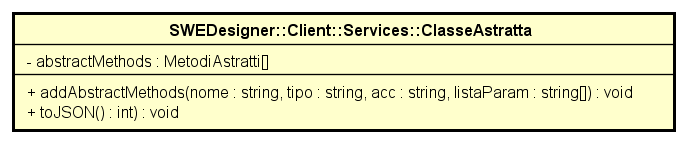
\includegraphics[scale=0.8]{Classi/SWEDesigner__Client__Services__ClasseAstratta.png}
			\caption{Diagramma della classe SWEDesigner::Client::Services::ClasseAstratta}
 			\end{figure}
				\begin{itemize}
          			\item \textbf{Descrizione:}\\
          			Classe derivata da classe che definisce i metodi di settaggio e richiesta dei parametri di una classe astratta.
          			\item \textbf{Utilizzo:}\\
          			É istaziata dal framework Angular e i suoi metodi sono utilizzati dal model global.
          			\item \textbf{Attributi:}\\
          			\begin{itemize}
          				\item \emph{-abstractMethods: MetodiAstratti[]}\\
            			Contiene la lista dei metodi della classe
          			\end{itemize}
          			\item \textbf{Metodi:}\\
          			\begin{itemize}
          				\item \emph{+addAbstractMethods(nome: string, tipo: string, acc:string, listaParam: string[]): void}\\
          				Questo metodo aggiunge un metodo alla classe astratta
          				\item \textbf{Parametri:}\\
            				\begin{itemize}
            					\item \emph{nome: string}\\
            					Nome del metodo
            					\item \emph{tipo: string}\\
            					Tipo di ritorno del metodo
            					\item \emph{acc:string}\\
            					Visibilità del metodo
            					\item \emph{listaParam: string[]}\\
            					Lista dei parametri del metodo
            				\end{itemize}
          				\item \emph{+toJSON()): void}\\
          				Questo metodo effettua il parsing della classe selezionata e lo trasforma in JSON
          			\end{itemize}
          		\end{itemize}
          	\paragraph{SWEDesigner::Client::Services::Interface}
          	\begin{figure}[h!]
			\centering
			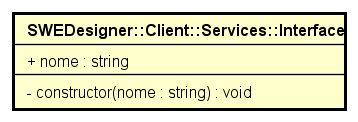
\includegraphics[scale=0.8]{Classi/SWEDesigner__Client__Services__Interface.png}
			\caption{Diagramma della classe SWEDesigner::Client::Services::Interface}
 			\end{figure}
				\begin{itemize}
          			\item \textbf{Descrizione:}\\
          			Classe derivata da classe che definisce i metodi di settaggio e richiesta dei parametri di una interface.
          			\item \textbf{Utilizzo:}\\
          			É istaziata dal framework Angular e i suoi metodi sono utilizzati dal model global.
          			\item \textbf{Attributi:}\\
          			\begin{itemize}
          				\item \emph{+nome: string}
          				Nome dell'Interfaccia
          			\end{itemize}
          			\item \textbf{Metodi:}\\
          			\begin{itemize}
          				\item \emph{-constructor(nome: string): void}
          				Costruttore
          				\item \textbf{Parametri:}\\
            				\begin{itemize}
            					\item \emph{nome: string}\\
            					Nome dell'interfaccia
            				\end{itemize}
          			\end{itemize}
          		\end{itemize}
          	\paragraph{SWEDesigner::Client::Services::Global}
          	\begin{figure}[h!]
			\centering
			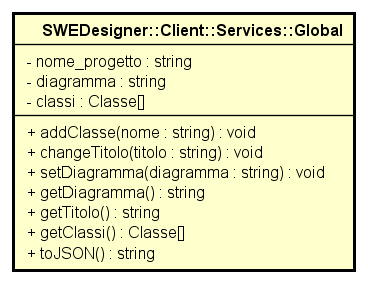
\includegraphics[scale=0.8]{Classi/SWEDesigner__Client__Services__Global.png}
			\caption{Diagramma della classe SWEDesigner::Client::Services:::Global}
 			\end{figure}
				\begin{itemize}
          			\item \textbf{Descrizione:}\\
          			Classe che definisce i metodi di settaggio e richiesta di tutte le classi contenenti nel diagramma delle classi.
          			\item \textbf{Utilizzo:}\\
          			É istaziata dal framework Angular e i suoi metodi sono utilizzati dal servizio editorService.
          			\item \textbf{Attributi:}\\
          			\begin{itemize}
          				\item \emph{-nomeprogetto: string}\\
          				Nome del progetto
          				\item \emph{-diagramma: string}\\
          				JSON convertito in string del diagramma
          				\item \emph{-classi: Classe[]}\\
          				Array di classi
          			\end{itemize}
          			\item \textbf{Metodi:}\\
          			\begin{itemize}
          				\item \emph{+addClasse(nome: string): void}\\
          				Nome del progetto
          				\item \emph{+changeTitolo(titolo: string): void}\\
          				JSON convertito in string del diagramma
          				\item \emph{+setDiagramma(diagramma: string): void}\\
          				Setta l'attributo diagramma della classe
          				\item \textbf{Parametri:}\\
            				\begin{itemize}
            					\item \emph{diagramma: string}\\
            					Diagramma
            				\end{itemize}
          				\item \emph{+getDiagramma(): string}\\
          				Ritorna il diagramma del progetto
          				\item \emph{+getTitolo(): string}\\
          				Ritorna il nome del progetto
          				\item \emph{+getClassi(): Classe[]}\\
          				Ritorna la collezione di classi
          				\item \emph{+toJSON(): string}
          				Ritorna un JSON del progetto in formato string
          			\end{itemize}
          		\end{itemize}
